Following are a few examples of queries and the results obtained using git commands and \gql.

\subsection{Query 1}
\textit{Find all the commits that affected a method foo.} \\
This command would involve a semantic search to identify the scope of a method block. However, neither git commands nor \gql search based on the syntax of the program. \\
Following are the two ways that can be used currently for this query.\\
\begin{description}
\item[1]. Use git grep to search for all the versions of find that contains the method foo and manually look at all the differences to identify if the method was changed.
\item[2]. Use git log with -L option that searches the history of a range of lines specified by a start and an end. But this range will change when lines are added or deleted around the method, and therefore every time a new commit affects the lines around the method; the query will change.
%The start and end parameters could also be a regex instead of the line number. \\ {\tt git log -L /foo/, /\}/:file.java}
\end{description}
When a method is added, a new choice is created between an empty string and the method. Further changes to this method will cause nested choices to be added in the right alternative of the initial choice. Therefore, the result of the above query is to find a choice and that introduced foo and then look for all the nested choices in the right alternative. \\
Following is the syntax of the queries in \gql.
\begin{description}
\item[] TO count number of commits that changed the method foo % \textit vs. \\
\begin{lstlisting}
 count (vgrep d$\langle$,*foo*$\rangle$ vs)
\end{lstlisting}
\item[] To show all the changes made to the method foo.
\begin{lstlisting}
 pretty (vgrep d$\langle$,*foo*$\rangle$ vs)
\end{lstlisting}
\item[] To further query the results
\begin{lstlisting}
vgrep pat from (vgrep d$\langle$,*foo*$\rangle$ vs)
\end{lstlisting}
\end{description}

\subsection{Query 2}
Were all the occurrences of a method name changed from 'foo' to 'bar'?

The distributive nature of git enables developers to work offline and then merge their commits. Sometimes this leads to merging conflicts that need to be resolved manually. Say, There were multiple branches created from the master at which point the method name was foo. Each branch renames the method differently, and while merging, one of the names is chosen, say 'bar'. To check if there are any occurrences of foo that was not merged correctly, the user would have to search for each of the different names. 

The following command in \gql can easily find all the occurrences that was not renamed from foo to bar.\\
\begin{lstlisting}
filter ("bar" `notIn` $ \$x $) from vgrep d$\langle$foo,$ \$x $ $\rangle$ vs
\end{lstlisting}

Here, the query first finds all the renames of foo and then filters the results based on whether the right alternative consists of bar or not. 
 










\begin{comment}
\subsection{Example 1}\label{ssec:ex1}
    
    Consider the following query - \\
    \textit{Find all the versions that consists of the function "foo"} \\
    There are two possible solutions to this query.
    \begin{description}
     \item[1] The following nested git command can be run. Such a command is not intuitive and requires a deeper understanding of the git command structure.
        \begin{lstlisting}
 git rev-list --all | GIT_PAGER=cat xargs git grep 'foo' 
        \end{lstlisting}
     \item[2] The brute force approach - a script to run grep on each version of the file by retrieving them one by one.
    \end{description}
    \subsection{Example 2}\label{ssec:ex2}
    Consider the following query - \\
    \textit{Find the commits that changed \tt{int} to \tt{long} }\\
    \\[2mm]
    The above query is to look for commit that changed the occurrence(s) of {\tt{int}} to {\tt{long}}.
    Using git commands, one can only find the commits that deleted {\tt{int}} and commits that added {\tt{long}} anywhere in the file. Both these results could point to different positions within the file.
    Figure ~\ref{fig:diff} is an example where the query should match the first change and not the other two.
    \begin{figure}
    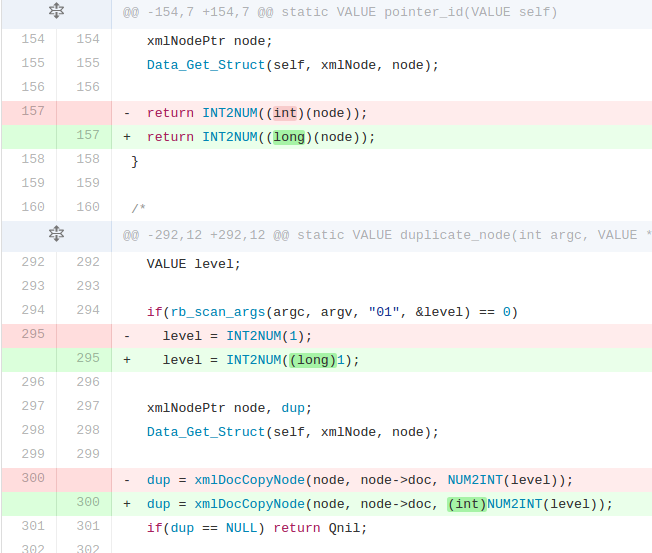
\includegraphics[width=\columnwidth]{diff}
    \caption{A commit that changed {\tt{int}} to \tt{long}}\label{fig:diff}
\end{figure}

gitQL is aimed at making such queries intuitive. It provides "choice pattern" constructs to specify the pattern for variations.
\end{comment}

\begin{comment}
Consider a scenario where a file consists of a function named foo. A branch is created from the main branch to add a different implementation of foo called baz while retaining foo. The user now decides to rename all the calls to foo to baz. 
Meanwhile, the function name foo its function calls were changed to bar in the main branch. 
Now, the newer implementation baz is better and tested thoroughly, and the developer decides to merge it. While merging the new implementation, of course, there is merge conflict and so the user resolves it by changing the function calls to bar to baz so as to retain the older function bar.

In the main branch, the function calls were changed from foo to bar and then again from bar to baz. 
At a later point, the software behaves funnily because some of the calls were still being made to bar. Therefore, the users want to look up all the places where the call to bar was not changed to baz. 

Using git commands, one will only find the versions that renamed foo to bar.  But we need all the subsequent changes in order to identify
\end{comment}